%=======================================================================
% Pipeline self-test preamble (English edition) -- not a real report
% Build: xelatex twice from selftest/en/
%=======================================================================
\documentclass[11pt,openany]{article}

% Latin text fonts
\usepackage{fontspec}
\setmainfont{Times New Roman}[Ligatures=TeX]
\setsansfont{Microsoft YaHei}
\setmonofont{Consolas}[Scale=0.86]

% CJK fallback: the self-test edition is English-only, but the shared preamble
% and the code listings may still carry Chinese comments.
\usepackage{xeCJK}
\setCJKmainfont{SimSun}[BoldFont=SimHei,ItalicFont=KaiTi]
\setCJKmonofont{FangSong}
\xeCJKsetup{CJKmath=false}

% =====================================================================
%  preamble-common.tex
%  Shared preamble for the RetNet-272M technical report (Chinese and
%  English editions).  Build with XeLaTeX.
%
%  Typographic convention (deliberately plain, single column, as in a
%  conventional technical report):
%    * serif body text, no coloured display headings
%    * numbered tables and figures, each with a caption
%    * remarks set as an indented, labelled passage rather than a
%      coloured box
% =====================================================================

\usepackage{amsmath}
\usepackage{amssymb}
\usepackage{bm}

% ---------- layout ---------------------------------------------------
\usepackage[a4paper,top=2.5cm,bottom=2.5cm,left=2.4cm,right=2.4cm]{geometry}
\usepackage{fancyhdr}
\usepackage{titlesec}
\usepackage{enumitem}
\usepackage{booktabs}
\usepackage{array}
\usepackage{tabularx}
% A table taller than a page must be able to break across pages: an unbreakable
% `tabular` that large is shipped out past the paper edge (Overfull \vbox), and
% the part below the edge is what the reader loses.  `longtable` is used only
% for such tables (see mktex.render_table).
\usepackage{longtable}
\usepackage{ragged2e}
\usepackage{xcolor}
\usepackage{caption}
\usepackage{graphicx}

% ---------- code -----------------------------------------------------
\usepackage{listings}
\usepackage{newunicodechar}

% ---------- references ----------------------------------------------
\usepackage[hidelinks,bookmarksnumbered]{hyperref}
\usepackage{bookmark}

% ---------- colours (used sparingly: code and rules only) ------------
\definecolor{codebg}{RGB}{248,248,249}
\definecolor{codeframe}{RGB}{216,220,225}
\definecolor{codecomment}{RGB}{104,124,108}
\definecolor{codekeyword}{RGB}{0,80,150}
\definecolor{codestring}{RGB}{160,60,40}
\definecolor{rulecol}{RGB}{178,182,188}
\definecolor{headrule}{RGB}{40,48,60}

% ---------- spacing --------------------------------------------------
\linespread{1.04}
\setlength{\parskip}{0.30em}
\setlength{\parindent}{0pt}
\setlength{\abovedisplayskip}{6pt}
\setlength{\belowdisplayskip}{6pt}
\setlength{\abovedisplayshortskip}{4pt}
\setlength{\belowdisplayshortskip}{4pt}

% Mixed CJK / monospace prose has few hyphenation opportunities; give TeX
% more room to stretch instead of leaving overfull boxes.
\tolerance=3000
\emergencystretch=3em
\hyphenpenalty=50
\hbadness=10000

% ---------- headings: plain, black, not coloured ---------------------
\titleformat{\section}
  {\normalfont\large\bfseries}{\thesection}{0.7em}{}
\titleformat{\subsection}
  {\normalfont\normalsize\bfseries}{\thesubsection}{0.7em}{}
\titleformat{\subsubsection}
  {\normalfont\normalsize\itshape}{\thesubsubsection}{0.7em}{}
\titlespacing*{\section}{0pt}{1.5em}{0.55em}
\titlespacing*{\subsection}{0pt}{1.05em}{0.40em}
\titlespacing*{\subsubsection}{0pt}{0.85em}{0.30em}

% ---------- header / footer ------------------------------------------
\pagestyle{fancy}
\fancyhf{}
\renewcommand{\headrulewidth}{0pt}
\renewcommand{\footrulewidth}{0pt}
\fancyfoot[C]{\small\thepage}

% ---------- tables and figures ---------------------------------------
\renewcommand{\arraystretch}{1.18}
\setlength{\tabcolsep}{5pt}
\captionsetup{
  font=small,
  labelfont=bf,
  labelsep=period,
  justification=raggedright,
  singlelinecheck=false,
  skip=5pt,
}
\captionsetup[table]{position=top}
\captionsetup[figure]{position=bottom}

% A numbered table with its caption above, as in the reference report.
\newenvironment{reporttable}[1]
  {\begin{center}\small\captionof{table}{#1}}
  {\end{center}}
\newcommand{\tabnote}[1]{\par\vspace{2pt}{\footnotesize #1}}

% ---------- lists ----------------------------------------------------
\setlist[itemize]{topsep=0.25em,itemsep=0.12em,parsep=0.08em,leftmargin=1.5em}
\setlist[enumerate]{topsep=0.25em,itemsep=0.12em,parsep=0.08em,leftmargin=1.8em}

% ---------- inline code ----------------------------------------------
\newcommand{\code}[1]{\texttt{\small #1}}
\newcommand{\file}[1]{\texttt{\small #1}}

% ---------- code listings --------------------------------------------
\lstdefinestyle{report}{
  backgroundcolor=\color{codebg},
  basicstyle=\ttfamily\fontsize{8.1}{9.6}\selectfont,
  commentstyle=\color{codecomment}\itshape,
  keywordstyle=\color{codekeyword}\bfseries,
  stringstyle=\color{codestring},
  frame=single,
  rulecolor=\color{codeframe},
  framesep=5pt,
  framexleftmargin=5pt,
  xleftmargin=5pt,
  breaklines=true,
  breakatwhitespace=false,
  breakindent=1.2em,
  columns=fullflexible,
  keepspaces=true,
  showstringspaces=false,
  tabsize=4,
  aboveskip=0.6em,
  belowskip=0.6em,
  upquote=true,
  extendedchars=true,
  inputencoding=utf8,
  escapechar=|,
  texcl=false,
  literate=%
    {→}{{$\rightarrow$}}1
    {←}{{$\leftarrow$}}1
    {×}{{$\times$}}1
    {÷}{{$\div$}}1
    {≈}{{$\approx$}}1
    {≤}{{$\leq$}}1
    {≥}{{$\geq$}}1
    {≠}{{$\neq$}}1
    {µ}{{$\mu$}}1
    {γ}{{$\gamma$}}1
    {Δ}{{$\Delta$}}1
    {σ}{{$\sigma$}}1
    {τ}{{$\tau$}}1
    {Σ}{{$\Sigma$}}1
    {√}{{$\surd$}}1
    {·}{{$\cdot$}}1
    {−}{{$-$}}1
    {∈}{{$\in$}}1
    {±}{{$\pm$}}1
    {∞}{{$\infty$}}1
    {❌}{{$\times$}}1
    {✅}{{$\checkmark$}}1
    {⚠}{{!}}1
}
\lstset{style=report}

% `listings` ships no PowerShell dialect; define just enough to colour it.
\lstdefinelanguage{PowerShell}{
  morekeywords={if,else,elseif,foreach,for,while,function,param,return,
    try,catch,finally,switch,break,continue,throw,in,not,and,or},
  sensitive=false,
  morecomment=[l]{\#},
  morestring=[b]",
  morestring=[b]',
}
\lstdefinelanguage{text}{}

% ---------- remarks --------------------------------------------------
% The source uses block quotes for asides.  They are set as an indented
% passage introduced by "Note." rather than as a coloured box.
\newenvironment{notebox}
  {\par\vspace{0.35em}%
   \begin{list}{}{%
     \setlength{\leftmargin}{1.5em}\setlength{\rightmargin}{0.4em}%
     \setlength{\topsep}{0pt}\setlength{\parskip}{0.25em}%
     \setlength{\parsep}{0.25em}\setlength{\itemsep}{0pt}%
     \setlength{\listparindent}{0pt}}%
   \item\relax\textbf{Note.}\ \ignorespaces}
  {\end{list}\vspace{0.15em}}

% ---------- rule -----------------------------------------------------
\newcommand{\reportrule}{\par\vspace{0.5em}{\color{rulecol}\hrule height 0.4pt}\vspace{0.7em}\par}

% ---------- appendices -----------------------------------------------
% The source writes the appendix titles with their letter already in the
% text ("Appendix A: Reproduction"), so the appendix section counter prints
% the letter and the *headings* of the back matter use a second counter that
% renumbers (Reference Reliability Note, References).
\newcounter{backmatter}
\newcommand{\startappendix}{%
  \clearpage
  \setcounter{section}{0}%
  \setcounter{backmatter}{0}%
  \renewcommand{\thesection}{\Alph{section}.}%
  % subsections are numbered against the appendix letter, so pin the format
  % explicitly: leaving \thesubsection as \thesection.\arabic{subsection}
  % would print `B..1' because \thesection already ends in a period.
  \renewcommand{\thesubsection}{\Alph{section}.\arabic{subsection}}%
}
\newcommand{\backmattersection}[1]{%
  \refstepcounter{backmatter}%
  \section*{\arabic{backmatter}.\quad #1}%
  \addcontentsline{toc}{section}{\protect\numberline{\arabic{backmatter}.}#1}%
}


\hypersetup{
  pdftitle  = {LaTeX Pipeline Self-Test},
  pdfauthor = {RetNet Project},
  pdfsubject= {LaTeX pipeline self-test},
}

\fancyhead[L]{\small\itshape LaTeX Pipeline Self-Test}
\fancyhead[R]{\small\thepage}
\fancyfoot[C]{}

\begin{document}


%=======================================================================
% Pipeline self-test title block and abstract (English edition)
% Inserted before the body; the body comes from en/_supplement.tex
%=======================================================================
\thispagestyle{empty}

\begin{center}
\vspace*{3.2cm}

{\LARGE\bfseries LaTeX Pipeline Self-Test}

\vspace{0.55cm}

{\large A placeholder document for the RetNet report pipeline}

\vspace{1.1cm}

{\normalsize RetNet Project}

\vspace{0.25cm}

{\small\itshape 2026-10-13}

\vspace{2.2cm}

\begin{minipage}{0.80\textwidth}
\centering\small
\begin{tabular}{@{}rl@{}}
\toprule
Purpose & exercises "Chinese-only Markdown $\rightarrow$ Chinese PDF" and \\
        & "hand-written supplement $\rightarrow$ English PDF" \\
Model & 504.18M parameters, 20 layers, 1408 wide, 22 heads (placeholder) \\
Data & 552.33M tokens $\times$ 3 epochs (placeholder) \\
\bottomrule
\end{tabular}
\end{minipage}

\vfill

{\small\itshape This PDF is a self-test artefact, not a deliverable.}

\vspace{1.2cm}
\end{center}

\clearpage

%-----------------------------------------------------------------------
% Abstract
%-----------------------------------------------------------------------
\section*{Abstract}
\addcontentsline{toc}{section}{Abstract}

This document exists only to exercise the build pipeline. Its Chinese edition is generated
from a Chinese-only Markdown file, and this English edition is generated in full from a
hand-written supplement. Every number quoted here is copied from the 0.5B fact sheet, which
was itself read out of the real \code{trainer\_state.json} files; nothing here is invented.

\clearpage

%-----------------------------------------------------------------------
% Contents
%-----------------------------------------------------------------------
\renewcommand{\contentsname}{Contents}
\tableofcontents

\clearpage


%=======================================================================
% Pipeline self-test -- English body (not a real report)
%
% Every number below is copied from docs/_report_0p5b/facts.md, which was read
% out of the real trainer_state.json files.
%=======================================================================

\section{Introduction}

This supplement is the whole English body of the self-test document. It exists to prove that
the English edition of a Chinese-only report can be built from a hand-written supplement, with
the same structure as the Chinese edition: the same sections in the same order, the same
tables, and the same figure.

The 0.5B model has 504{,}179{,}896 parameters (504.18M) in 20 layers of width 1408 with 22
heads, and was trained for three legs over the same 552.33M-token packed corpus, one epoch per
leg. The pipeline under test must render all of that without inventing anything.

\subsection{Configuration}

\begin{center}\small
\captionof{table}{Model configuration}
\begin{tabular}{@{}>{\RaggedRight\arraybackslash}p{0.34\textwidth}>{\RaggedRight\arraybackslash}p{0.58\textwidth}@{}}
\toprule
\textbf{Item} & \textbf{Value} \\
\midrule
Parameters & \textbf{504{,}179{,}896} (504.18M) \\
Layers / width / heads & 20 / 1408 / 22 \\
Feed-forward and value width & 2816 / 2816 \\
Vocabulary & 20{,}000 (tied embeddings) \\
Retention mode & \code{chunkwise}, \code{chunk\_size} 128 \\
Learned per-head decay gate & enabled (\code{use\_gla}) \\
Growth layer norm & enabled, \code{growth\_old\_dim} 768 \\
Storage precision & \code{float32} in \code{config.json}; trained in bf16 \\
\bottomrule
\end{tabular}
\end{center}

\section{Training}

The three legs share one corpus and one schedule shape: every leg restarts a full cosine with a
peak of $1.1\times10^{-4}$ and 500 warm-up steps, rather than continuing from the previous leg's
learning-rate tail.

\subsection{Training Legs}

\begin{center}\small
\captionof{table}{The three training legs}
\begin{tabular}{@{}llrrr@{}}
\toprule
\textbf{Leg} & \textbf{Hardware} & \textbf{Steps} & \textbf{Tokens per step} & \textbf{Total tokens} \\
\midrule
ep1 & RTX 3090 24\,GB & 67{,}390 & 8{,}192 & 552{,}058{,}880 \\
ep2 & RTX PRO 6000 & 16{,}848 & 32{,}768 & 552{,}140{,}800 \\
ep3 & RTX PRO 6000 & 16{,}848 & 32{,}768 & 552{,}140{,}800 \\
\bottomrule
\end{tabular}
\end{center}

Cumulatively the three legs consumed 1{,}656{,}340{,}480 tokens, or 3.285 tokens per parameter.

\subsection{Validation Loss}

\begin{center}\small
\captionof{table}{Validation loss of the three legs}
\begin{tabular}{@{}lrrr@{}}
\toprule
\textbf{Leg} & \textbf{First eval} & \textbf{Best eval} & \textbf{Best step} \\
\midrule
ep1 & 2.6358 & \textbf{2.1035} & 65{,}000 \\
ep2 & 2.1800 & \textbf{1.9865} & 16{,}848 \\
ep3 & 2.1174 & \textbf{1.9459} & 16{,}848 \\
\bottomrule
\end{tabular}
\end{center}

\subsection{The Cost of the Hot Restarts}

\begin{figure}[htbp]
\centering
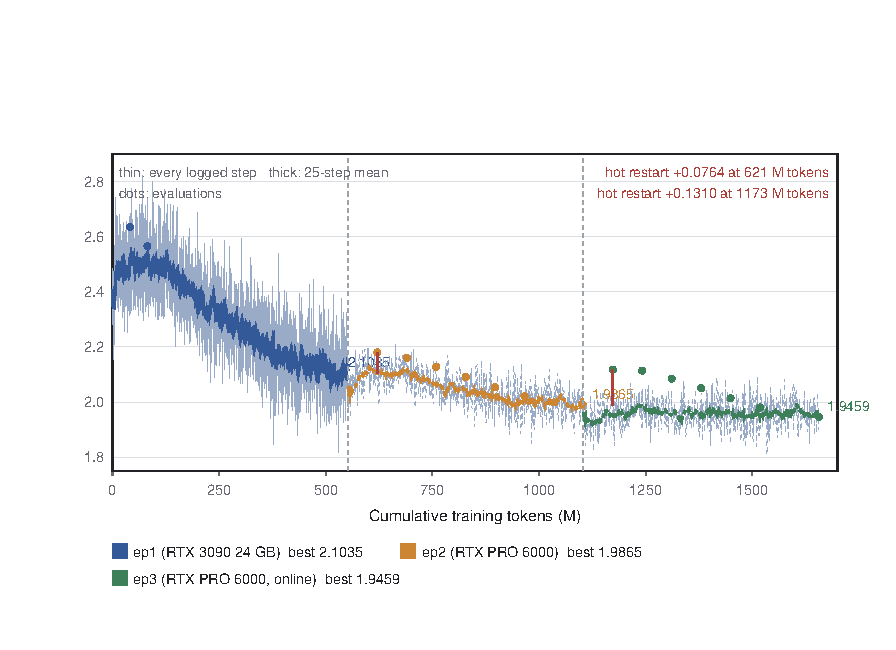
\includegraphics[width=\linewidth]{../../figures/fig-0p5b-loss}
\caption{Validation loss of the three training legs. The thin line is every logged step, the thick line its 25-step rolling mean, and the dots are the evaluations; every leg restarts a full cosine. Source: the three \code{trainer\_state.json} files.}
\label{fig:fig-0p5b-loss}
\end{figure}

\begin{figure}[htbp]
\centering
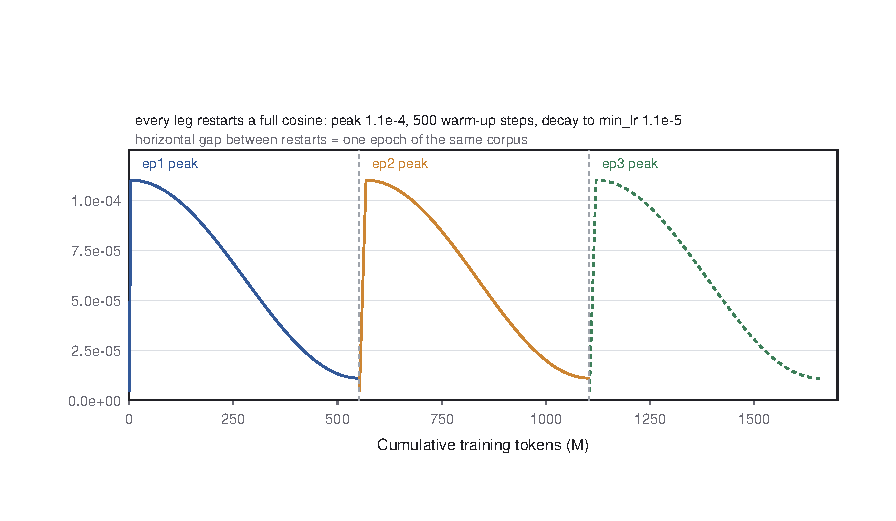
\includegraphics[width=\linewidth]{../../figures/fig-0p5b-lr}
\caption{Learning rate of the three legs: every leg restarts a full cosine (peak $1.1\times10^{-4}$, 500 warm-up steps, decay to \code{min\_lr} $1.1\times10^{-5}$) instead of continuing from the previous leg's tail. Same source as the loss figure.}
\label{fig:fig-0p5b-lr}
\end{figure}

\begin{center}\small
\captionof{table}{Cost of the hot restarts}
\begin{tabular}{@{}lrrr@{}}
\toprule
\textbf{Hand-off} & \textbf{Previous best} & \textbf{Next first eval} & \textbf{Difference} \\
\midrule
ep1 $\rightarrow$ ep2 & 2.1035 @65{,}000 & 2.1800 @2{,}106 & $+0.0764$ \\
ep2 $\rightarrow$ ep3 & 1.9865 @16{,}848 & 2.1174 @2{,}106 & $+0.1310$ \\
\bottomrule
\end{tabular}
\end{center}

Both hand-offs made the model \emph{worse} before it recovered: the first evaluation of a new
leg sits above the previous leg's best, by 0.0764 and 0.1310 respectively, and both legs do
eventually finish below that starting point.

\startappendix
\section{Appendix A: Reproduction}

\begin{lstlisting}[language=Python]
# 1) the figures, from the real state files
python makefigs.py

# 2) Markdown -> LaTeX, then two XeLaTeX passes per edition
python mktex.py --report selftest
\end{lstlisting}

\backmattersection{References}

\begin{itemize}
  \item Retentive Network: A Successor to Transformer for Large Language Models. arXiv:2307.08621.
  \item Gated Linear Attention Transformers with Hardware-Efficient Training. arXiv:2312.06635.
\end{itemize}

\end{document}
